% ============================================================
%  Balancing Robot – API & Benutzerhandbuch
%  Design: AR10-inspiriert, kompakter Referenz-Stil
%  Compiler: pdflatex (2× laufen lassen)
% ============================================================

\documentclass[11pt, a4paper]{scrartcl}

\usepackage[T1]{fontenc}
\usepackage[utf8]{inputenc}
\usepackage[ngerman]{babel}
\usepackage{lmodern}
\usepackage{microtype}

\usepackage[a4paper,
  top=25mm, bottom=28mm,
  left=20mm, right=20mm,
  includeheadfoot]{geometry}

\usepackage{xcolor}
\usepackage{graphicx}
\usepackage{tikz}
\usetikzlibrary{calc}
\usepackage{tcolorbox}
\tcbuselibrary{skins, breakable, listings}
\usepackage{titlesec}
\usepackage{fancyhdr}
\usepackage{enumitem}
\usepackage{booktabs}
\usepackage{multicol}
\usepackage{hyperref}
\usepackage{listings}

% Farben
\definecolor{htbblue}{HTML}{0078C8}
\definecolor{htbdark}{HTML}{003E6B}
\definecolor{htblight}{HTML}{E8F4FC}
\definecolor{htbgray}{HTML}{F4F4F4}
\definecolor{htbtextgray}{HTML}{555555}
\definecolor{htbgreen}{HTML}{2ECC71}
\definecolor{htbred}{HTML}{E74C3C}

\usepackage{helvet}
\renewcommand{\familydefault}{\sfdefault}

\hypersetup{
  colorlinks=true,
  linkcolor=htbblue,
  urlcolor=htbblue,
  pdftitle={Balancing Robot – API \& Benutzerhandbuch},
}

% ── Code-Listings ────────────────────────────────────────────
\lstset{
  language=Python,
  basicstyle=\ttfamily\small,
  keywordstyle=\color{htbblue}\bfseries,
  commentstyle=\color{htbtextgray}\itshape,
  stringstyle=\color{htbdark},
  backgroundcolor=\color{htbgray},
  frame=tb, framerule=0pt,
  numbers=left, numberstyle=\tiny\color{htbtextgray},
  breaklines=true,
  showstringspaces=false,
  tabsize=4,
}

% ── Kopfzeile ────────────────────────────────────────────────
\pagestyle{fancy}
\fancyhf{}
\renewcommand{\headrulewidth}{0pt}
\fancyhead[L]{%
  \begin{tikzpicture}[remember picture, overlay]
    \fill[htbblue] (0,0) rectangle (\textwidth+4mm, 7mm);
    \node[anchor=west, white, font=\small\bfseries] at (2mm,3.5mm)
      {Balancing Robot – API \& Benutzerhandbuch};
    \node[anchor=east, white, font=\small] at (\textwidth+2mm,3.5mm)
      {\thepage};
  \end{tikzpicture}%
}
\setlength{\headheight}{10mm}

\fancypagestyle{plain}{%
  \fancyhf{}
  \renewcommand{\headrulewidth}{0pt}
  \fancyfoot[C]{\color{htbtextgray}\small\thepage}
}

% ── Abschnittsüberschriften ──────────────────────────────────
\titleformat{\section}
  {\color{htbblue}\Large\bfseries}
  {\thesection}
  {1em}{}
  [\color{htbblue}\titlerule[1pt]]

\titleformat{\subsection}
  {\color{htbdark}\large\bfseries}
  {\thesubsection}
  {1em}{}

\titleformat{\subsubsection}
  {\color{htbdark}\normalsize\bfseries}
  {}
  {0pt}{}

% ── Boxen ────────────────────────────────────────────────────

% API-Klassen/Funktions-Box (blauer Header)
\newtcolorbox{apibox}[2][]{
  enhanced, breakable,
  colback=htbgray, colframe=htbblue,
  colbacktitle=htbblue, coltitle=white,
  fonttitle=\ttfamily\bfseries,
  title={#2},
  sharp corners,
  left=4mm, right=4mm,
  #1
}

% Hinweis-Box
\newtcolorbox{notebox}{
  enhanced,
  colback=htblight, colframe=htbblue,
  leftrule=4pt, toprule=0pt, bottomrule=0pt, rightrule=0pt,
  sharp corners,
}

% Warnung-Box
\newtcolorbox{warnbox}{
  enhanced,
  colback=yellow!10, colframe=orange!80!black,
  leftrule=4pt, toprule=0pt, bottomrule=0pt, rightrule=0pt,
  sharp corners,
}

% Parameter-Tabelle in API-Box
\newcommand{\apiparam}[3]{%
  \texttt{#1} & \texttt{\color{htbdark}#2} & #3 \\
}

% ── Titelseite (AR10-Stil) ───────────────────────────────────
\newcommand{\makeapititle}{%
  \begin{titlepage}
    \newgeometry{margin=0pt}
    \begin{tikzpicture}[remember picture, overlay]

      % Blauer oberer Block (55 %)
      \fill[htbblue]
        (current page.north west)
        rectangle
        ([yshift=-0.55\paperheight]current page.north east);

      % Roboterbild oben links
      \node[anchor=north west]
        at ([xshift=10mm, yshift=-8mm]current page.north west)
        {%
          \IfFileExists{robot_cover.png}{%
            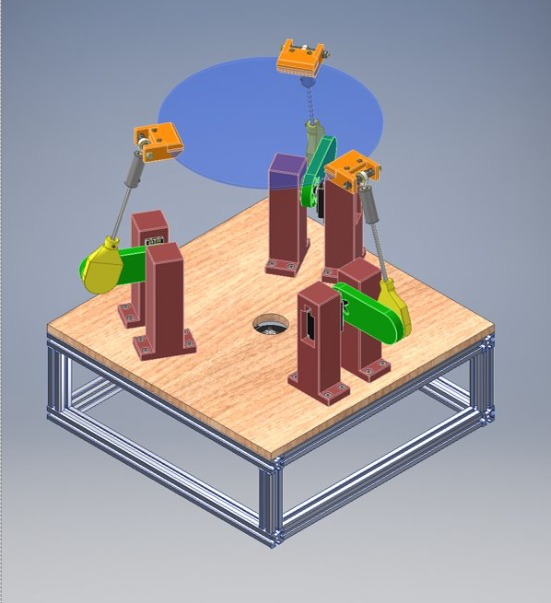
\includegraphics[width=90mm, keepaspectratio]{robot_cover.png}%
          }{%
            \IfFileExists{robot_cover.jpg}{%
              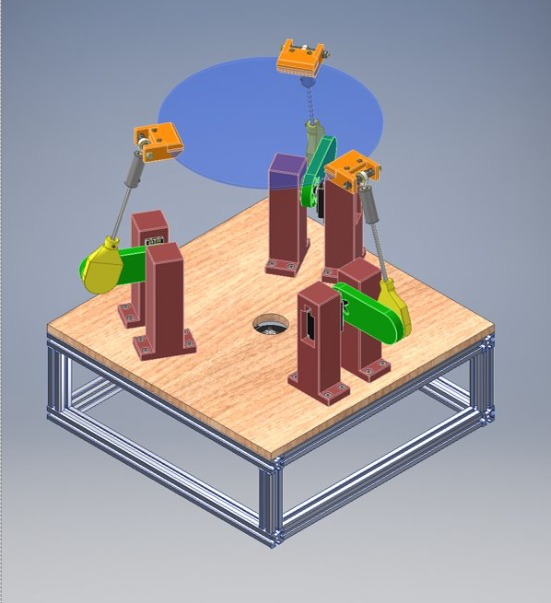
\includegraphics[width=90mm, keepaspectratio]{robot_cover.jpg}%
            }{%
              \begin{tikzpicture}
                \draw[white, dashed, line width=1pt, opacity=0.4]
                  (0,0) rectangle (90mm, 110mm);
                \node[white, opacity=0.5, font=\small] at (45mm,55mm)
                  {robot\_cover.png/.jpg};
              \end{tikzpicture}%
            }%
          }%
        };

      % Titel unten rechts im blauen Block
      \node[anchor=south east, align=right]
        at ([xshift=-14mm, yshift=12mm]current page.north east |-
            [yshift=-0.55\paperheight]current page.north)
        {%
          {\fontsize{36}{40}\selectfont\bfseries\color{white}Balancing Robot}\\[4pt]
          {\large\bfseries\color{white!85!htbblue}API \& Benutzerhandbuch}%
        };

      % Dokumenttyp + Projektname (weißer Bereich)
      \node[anchor=north west, align=left]
        at ([xshift=14mm, yshift=-10mm]current page.south west |-
            [yshift=-0.55\paperheight]current page.north)
        {%
          {\large\bfseries\color{black}API \& Benutzerhandbuch}\\[4pt]
          {\normalsize\color{htbtextgray}Balancing Robot · HTW Berlin · WiSe 2025/26}%
        };

      % HTW-Logo unten rechts
      \node[anchor=south east]
        at ([xshift=-14mm, yshift=14mm]current page.south east)
        {%
          \IfFileExists{htw_logo.png}{%
            
\includegraphics[height=18mm, keepaspectratio]{htw_logo.png}%
          }{%
            \begin{tikzpicture}
              \draw[htbblue, dashed, line width=0.8pt, opacity=0.5]
                (0,0) rectangle (40mm,16mm);
              \node[htbblue, opacity=0.6, font=\small] at (20mm,8mm)
                {htw\_logo.png};
            \end{tikzpicture}%
          }%
        };

    \end{tikzpicture}
    \restoregeometry
  \end{titlepage}
}

% ============================================================
\begin{document}

\makeapititle

\tableofcontents
\clearpage

% ============================================================
\section{Schnellstart}

\begin{notebox}
  Alle Beispiele laufen auf dem Laptop mit \texttt{MockServoDriver} —
  kein Raspberry Pi erforderlich.
\end{notebox}

\begin{lstlisting}[caption={Minimales Beispiel}]
from balancing_platform import Platform
from hardware import MockServoDriver

platform = Platform(MockServoDriver())
platform.neutral()
platform.set_tilt(winkel_x=5.0, winkel_y=-3.0)
platform.close()
\end{lstlisting}

% ============================================================
\section{Modul \texttt{balancing\_platform}}

\begin{apibox}{class Platform}
  Zentrale API für die Plattformsteuerung. Verbindet Inverse Kinematik
  mit dem Servo-Treiber.

  \medskip
  \textbf{Konstruktor}
  \begin{lstlisting}[numbers=none]
Platform(driver: ServoDriver, geometry: PlatformGeometry | None = None)
  \end{lstlisting}

  \medskip
  \textbf{Parameter}
  \smallskip

  \begin{tabular}{lll}
    \toprule
    Name & Typ & Beschreibung \\
    \midrule
    \apiparam{driver}{ServoDriver}{Servo-Treiber (Mock oder PCA9685)}
    \apiparam{geometry}{PlatformGeometry}{Maschinenparameter (optional)}
    \bottomrule
  \end{tabular}
\end{apibox}

\subsection{Methoden}

\begin{apibox}{platform.set\_tilt(winkel\_x, winkel\_y, ref\_point=None)}
  Neigt die Plattform um die angegebenen Winkel.

  \medskip
  \begin{tabular}{lll}
    \toprule
    Parameter & Typ & Beschreibung \\
    \midrule
    \apiparam{winkel\_x}{float}{Neigungswinkel um X-Achse [°]}
    \apiparam{winkel\_y}{float}{Neigungswinkel um Y-Achse [°]}
    \apiparam{ref\_point}{ndarray}{Referenzpunkt [mm], Standard: Plattformmitte}
    \bottomrule
  \end{tabular}

  \medskip
  \textbf{Rückgabe:} \texttt{KinematicsResult}
\end{apibox}

\begin{apibox}{platform.neutral()}
  Fährt alle Servos in die Neutralposition (Plattform waagerecht).
\end{apibox}

\begin{apibox}{platform.close()}
  Gibt Ressourcen frei. Alternativ als Context Manager nutzbar.
\end{apibox}

\begin{lstlisting}[caption={Context Manager}]
with Platform(PCA9685Driver.from_config("config.json")) as p:
    p.set_tilt(10, 0)
# close() wird automatisch aufgerufen
\end{lstlisting}

% ============================================================
\section{Modul \texttt{hardware}}

\begin{apibox}{class MockServoDriver}
  Simulierter Treiber für Tests ohne Hardware. Gibt Servowinkel
  auf der Konsole aus.

  \begin{lstlisting}[numbers=none]
MockServoDriver(verbose: bool = True)
  \end{lstlisting}
\end{apibox}

\begin{apibox}{class PCA9685Driver}
  Treiber für das PCA9685 I²C PWM-Board (nur Raspberry Pi).

  \begin{lstlisting}[numbers=none]
PCA9685Driver.from_config(path: str | Path) -> PCA9685Driver
  \end{lstlisting}

  Lädt Kanal- und Pulskonfiguration aus \texttt{config.json}.
\end{apibox}

\begin{warnbox}
  \textbf{Achtung:} \texttt{PCA9685Driver} importiert \texttt{adafruit\_servokit},
  das nur auf dem Pi verfügbar ist. Auf dem Laptop immer \texttt{MockServoDriver}
  verwenden.
\end{warnbox}

% ============================================================
\section{Modul \texttt{kinematik}}

\begin{apibox}{class KinematicsEngine}
  Berechnet Servowinkel aus Plattformneigung (Inverse Kinematik).

  \begin{lstlisting}[numbers=none]
engine = KinematicsEngine(geometry, solver_method="scipy")
result = engine.solve(winkel_x=5.0, winkel_y=-3.0)
  \end{lstlisting}
\end{apibox}

\begin{apibox}{dataclass KinematicsResult}
  \begin{tabular}{lll}
    \toprule
    Attribut & Typ & Beschreibung \\
    \midrule
    \apiparam{servo\_v}{float}{Servowinkel vorne [°]}
    \apiparam{servo\_l}{float}{Servowinkel links [°]}
    \apiparam{servo\_r}{float}{Servowinkel rechts [°]}
    \apiparam{actual\_angle\_x}{float}{Tatsächlicher Winkel X [°]}
    \apiparam{actual\_angle\_y}{float}{Tatsächlicher Winkel Y [°]}
    \apiparam{n\_vek}{ndarray}{Normalvektor der Plattform}
    \apiparam{d}{float}{Ebenenparameter d}
    \apiparam{solver\_success}{bool}{Konvergenz des Solvers}
    \apiparam{reachability\_ok}{bool}{Winkel im Erreichbarkeitsbereich}
    \bottomrule
  \end{tabular}
\end{apibox}

% ============================================================
\section{Modul \texttt{vision}}

\begin{apibox}{class BallDetectorRuntime}
  Echtzeiterfassung der Ballposition via Kamera (HSV-Filter + Kontursuche).

  \begin{lstlisting}[numbers=none]
detector = BallDetectorRuntime(hsv_range=HSV_RANGE, frame_size=(640,480))
detector.start()
frame = detector.get_latest_frame()
detector.stop()
  \end{lstlisting}
\end{apibox}

\begin{apibox}{class BallTracker}
  Schätzt Position und Geschwindigkeit des Balls aus Einzelmessungen.

  \begin{lstlisting}[numbers=none]
tracker = BallTracker(detector)
state = tracker.get()
# state.x, state.y    – Position [px von Bildmitte]
# state.vx, state.vy  – Geschwindigkeit [px/s]
# state.valid         – False wenn kein Ball sichtbar
  \end{lstlisting}
\end{apibox}

\begin{apibox}{dataclass HsvRange}
  HSV-Farbgrenzen für die Ballerkennung.

  \begin{lstlisting}[numbers=none]
HsvRange(lower=np.array([90, 80, 60]), upper=np.array([130, 255, 255]))
  \end{lstlisting}
  Werte werden mit \texttt{cv2.inRange} verglichen (OpenCV HSV: H 0–180).
\end{apibox}

% ============================================================
\section{Konfiguration}

\subsection{config.json}

\begin{lstlisting}[language={},caption={config.json Struktur}]
{
  "pca9685": {
    "address": "0x40",
    "channels": {
      "front": 0,
      "left":  1,
      "right": 2
    },
    "pulse_min_us": 500,
    "pulse_max_us": 2500
  },
  "servos": {
    "front": { "offset_deg": 20,  "modifier": 1.0  },
    "left":  { "offset_deg": 35,  "modifier": 1.0  },
    "right": { "offset_deg": 20,  "modifier": 1.05 }
  }
}
\end{lstlisting}

\subsection{positions.json (Kalibrierung)}

\begin{lstlisting}[language={},caption={positions.json für capture\_calibration\_set.py}]
{
  "positions": [
    { "name": "center",   "roll_deg": 0,  "pitch_deg": 0  },
    { "name": "tilt_p5x", "roll_deg": 0,  "pitch_deg": 5  },
    { "name": "tilt_n5x", "roll_deg": 0,  "pitch_deg": -5 }
  ]
}
\end{lstlisting}

% ============================================================
\section{Inbetriebnahme}

\subsection{Voraussetzungen}

\begin{itemize}[leftmargin=*]
  \item Python 3.11+
  \item Pakete: \texttt{pip install numpy opencv-python numba scipy adafruit-circuitpython-servokit}
  \item Für Pi: I²C aktiviert (\texttt{raspi-config})
\end{itemize}

\subsection{Laptop-Test}

\begin{lstlisting}[caption={Kinematik-Test ohne Hardware}]
python -m pytest tests/platform_mock_test.py -v
\end{lstlisting}

\subsection{Start auf dem Raspberry Pi}

\begin{lstlisting}[caption={Regelloop starten}]
# In main_control.py: MockServoDriver durch PCA9685Driver ersetzen
python main_control.py
\end{lstlisting}

\subsection{Kamerakalibrierung}

\begin{lstlisting}[caption={Kalibrierbilder aufnehmen}]
cd vision/calibration
python capture_calibration_set.py   # Schachbrett auf Plattform legen
python run_calibration.py           # camera_matrix.npz erzeugen
\end{lstlisting}

\end{document}
